%+================+
%| DOCUMENT SETUP |
%+================+

% Set document class
\documentclass[xcolor=dvipsnames,11pt,paper=a4paper]{report}

% Include packages
\usepackage[utf8]{inputenc}
\usepackage[T1]{fontenc}
\usepackage[ngerman]{babel}
\usepackage{graphicx}
\usepackage{xcolor}
\usepackage{listings}
\usepackage{fancyhdr}
\usepackage{tikz}
\usepackage{hyperref}
\lstdefinelanguage{javascript}{
  keywords={abstract, public, break, case, catch, continue, debugger, default, delete, do, else, finally, for, function, if, in, instanceof, new, null, return, switch, throw, try, typeof, var, void, while, with},
  keywords={[2]{class, export, boolean, String, Date, Infinity, Number, throw, implements, import, this, undefined, false, true, byte, int, document}},
  sensitive=false,
  comment=[l]{//},
  morecomment=[s]{/*}{*/},
  morestring=[b]',
  morestring=[b]"
}
\lstdefinelanguage{svg}{
	keywords={svg, circle, line, polygon, rectangle},
	keywords={[2]{width, height, viewBox, cx, cy, r, x1, x2, y1, y2, xmlns, stroke-width, stroke-linecap, stroke-linejoin, stroke, fill}},
	alsoletter=-,
	sensitive=false,
	comment=[l]{//},
	morecomment=[s]{/*}{*/},
	morestring=[b]',
	morestring=[b]"
}
\lstdefinelanguage{json}{
    sensitive=false,
    morestring=[b]',
    morestring=[b]",
    literate=
    {[}{{\color{red}\[}}1
}

\lstnewenvironment{code}[1][]{
	\lstset{
		#1,
		captionpos=b,
		backgroundcolor=\color{white},
		basicstyle=\footnotesize\ttfamily,
		commentstyle=\color{cyan}\itshape,
		keywordstyle=[1]\color{red}\bfseries,
		keywordstyle=[2]\color{violet}\bfseries,
		numberstyle=\color{black},
		stringstyle=\color{gray},
		breakatwhitespace=true,
		breaklines=true,
		keepspaces=true,
		numbers=left,
		numbersep=7pt,
		showspaces=false,
		showstringspaces=true,
		showtabs=false,
		tabsize=2,
		frame=l,
		extendedchars=true,
		literate=
		{Ö}{{\"O}}1
		{Ä}{{\"A}}1
		{Ü}{{\"U}}1
		{ß}{{\ss}}2
		{ü}{{\"u}}1
		{ä}{{\"a}}1
		{ö}{{\"o}}1
		{~}{{\textasciitilde}}1
	}
}{}		% Code style setup

%+----------------+
%| Document style |
%+----------------+

% Set default font to sans-serif
\renewcommand*{\familydefault}{\sfdefault}
% Make monospaced font a little smaller to fit text size
\let\tt\ttfamily
\renewcommand*{\ttfamily}{\small\tt}

% No horizontal paragraph indentation
\setlength{\parindent}{0pt}
\setlength{\parskip}{1em}

% Don't reset footnote counter with each chapter
\counterwithout{footnote}{chapter}

% Line spacing
\renewcommand{\baselinestretch}{1.5}

% Space before itemize/enumerate
\setlist[itemize]{topsep=-11pt}
\setlist[enumerate]{topsep=-11pt}

% Space after List of Figures etc.
\setlength\cftaftertoctitleskip{12pt}
\setlength\cftafterloftitleskip{12pt}
\setlength\cftafterlottitleskip{12pt}
\setlength{\cftbeforechapskip}{12pt}
\setlength{\cftbeforesecskip}{6pt}
\setlength{\cftbeforesubsecskip}{6pt}

% Set chapter style
\titleformat{\chapter}{\Huge\bfseries}{\thechapter. }{0pt}{\Huge\bfseries}
\titlespacing{\chapter}{0pt}{0pt}{20pt}
\titlespacing{\section}{0pt}{12pt}{0pt}
\titlespacing{\subsection}{0pt}{12pt}{0pt}
\titlespacing{\subsubsection}{0pt}{12pt}{0pt}

% Set author and title
\title{
	\Huge\textbf{Praxissemester bei isys vision GmbH \& Co. KG}\\\vspace{20pt}
	\huge{Bericht und Erfahrungen}
}
\author{
	\begin{tabular}{l l}
	Lorenz Bung &
	\href{mailto:lorenz.bung@htwg-konstanz.de}{\texttt{lorenz.bung@htwg-konstanz.de}}\\
	&HTWG Konstanz\\
	&Angewandte Informatik, 4. Semester
	\end{tabular}
}
\date{01. März 2018 bis 31. Juli 2018}

%+================+
%| DOCUMENT START |
%+================+
\begin{document}
\pagenumbering{gobble} % No page numbers for the introduction!

%+------------+
%| Title page |
%+------------+
\begin{titlepage}
\begin{tabular}{l r}

\includegraphics[width=0.5\textwidth]{media/htwg.png} &

\includegraphics[width=0.5\textwidth]{media/isys.png}
\end{tabular}
{\let\newpage\relax\maketitle}
\end{titlepage}

%+----------+
%| Abstract |
%+----------+
\begin{abstract}
In diesem Bericht geht es um mein Praktikum bei isys vision GmbH \& Co. KG, welches
ich im Rahmen meines Bachelorstudiums im Fach Angewandte Informatik im 4. Studiensemester
absolviert habe.

Ich werde beschreiben und erklären, welche Aufgaben mir weshalb gegeben wurden,
wie ich sie gelöst habe und welche Werkzeuge und Vorgehensweisen ich dabei verwendet
habe. Weiterhin werde ich die firmeninternen Abläufe, Ziele und Methoden nennen.
Die mir während dem Praktikum zugeteilten Aufgaben umfassten ein breites Spektrum mit dem Fokus
Webentwicklung und Javascript. Dabei war ich in mehreren Bereichen der Firma
tätig und bekam so ein umfassendes Bild der Arbeit.

Meine Tätigkeit umfasste die Modifikation eines bereits bestehenden Webinterfaces, die Einrichtung eines Datenbankservers und eines Projektmanagementsystems sowie den Aufbau eines Steuerungstools zur Kontrolle eines Roboters und eine WebGL-basierte Browseranwendung zur Vorschau von Punktwolken.

Abschließend werde ich ein Fazit aus den gesammelten Erfahrungen ziehen und positive
bzw. negative Aspekte meiner Tätigkeit hervorheben. Ich werde außerdem zusammenfassen,
inwiefern das Praxissemester mich weiter gebracht hat und mein akademisches Profil
durch praktische Erfahrung abrundet.
\end{abstract}
\pagebreak

%+-------------------+
%| Table of contents |
%+-------------------+
\tableofcontents
\pagebreak

%+-------------------+
%| List of Listings, |
%| List of Figures,  |
%| List of Tables    |
%+-------------------+
\begingroup
\let\clearpage\relax
\lstlistoflistings
\listoffigures
\listoftables
\endgroup
\pagebreak

%+------------+
%| Einleitung |
%+------------+
\pagenumbering{arabic} % turn page numbering on now
\setcounter{chapter}{-1} % Makes numbering start at 0, so ``real'' chapters start at 1.
\chapter{Einleitung}
\label{ch:0}

Zu Beginn möchte ich kurz die Hintergründe meines Praktikums erläutern,
z.B. einige Informationen zu isys vision, die Wahl der Firma und den Bewerbungsprozess.

isys vision\footnote{\url{http://www.isys-vision.de}} ist ein Softwarehersteller, der sich mit grafischen Lösungen im industriellen Einsatz auseinandersetzt.
Die Bildverarbeitung steht hierbei im Vordergrund und wird durch die von isys produzierte
Software durchgeführt. Es handelt sich hierbei um ein mittelständisches Unternehmen mit etwa 20 Mitarbeitern. Die im selben Gebäude gelegene Tochterfirma Ensenso\footnote{\url{http://www.ensenso.com}} stellt
Kamera- und Hardwarekomponenten her, welche dann in Kombination mit der Software von isys vision
als Gesamtpaket an Endkunden, aber auch Zulieferer und Großkunden verkauft wird. Dies umfasst
hauptsächlich Komponenten wie Kameras, Beleuchtungsbauteile und Verbindungskabel
sowie vollständige Rechensysteme, als auch die entwickelte Software.

Schon im Grundstudium war mir klar, dass ich für mein praktisches Studiensemester
Firmen im Bereich der Bildverarbeitung, -generierung oder aber im Webumfeld suchen
werde. Mit einem Praktikum in genannten Gebieten wollte ich einerseits meine Entscheidung
für die Vertiefungsrichtung der Medieninformatik im Hauptstudium bekräftigen, andererseits
war dies schon immer ein Bereich der Informatik, welcher mich besonders gereizt
hat. Aus diesen Gründen habe ich mich unter Anderem bei isys vision beworben und
schlussendlich ein halbes Jahr hier verbracht.





%+-----------+
%| Kapitel 1 |
%+-----------+
\chapter{Web-Oberfläche für das IVS}
\label{ch:ivs}

Das erste größere Projekt war die Entwicklung einer Web-Oberfläche für ein bereits
bestehendes, jedoch noch nicht vollständiges Bildverarbeitungssystem. Sowohl Webinterface
als auch Bildverarbeitung waren bereits vorhanden, jedoch nicht für den aktuellen
Anwendungszweck geeignet und somit war eine Überarbeitung unabdingbar.

Die Aufgabe des betreffenden Systems ist die Ausrichtung einzelner Keramikseiten,
welche dann in weiteren Schritten verarbeitet werden. Dabei geht es um die Produktion
von Lambdasonden, wie sie in der Abgasfilterung von Autos zum Einsatz kommen.

Diese Keramik-``sheets'' werden dabei mit hochpräziser Genauigkeit ausgestanzt,
weswegen sie vor dem Stanzen entsprechend ausgerichtet werden müssen. Eine physikalische
Ausrichtung ist dabei so gut wie unmöglich, da die gewünschte Genauigkeit dabei
nicht erreicht werden kann.

Das von isys entwickelte System erkennt nun mithilfe
zweier Kameras die Lage zweier Marken auf dem Sheet und somit die Lage auf dem verschieb-
und rotierbaren Tisch. Mithilfe der Bildverarbeitungssoftware wird nun eine Motorbewegung
errechnet, welche eine Ausrichtung des Werkstücks bewirkt. Anschließend kann das
Teil durch weitere Maschinen in seiner nun festgelegten Position weiterverarbeitet
werden.

Die Software besteht dabei nun aus drei verschiedenen Komponenten:
\begin{itemize}
	\item Dem \textit{ScbDrv}, welcher für die Ansteuerung der Motoren und Hardware
	verantwortlich ist.
	\item Dem \textit{IVS} (Isys Vision Server), welcher für die Auswertung der Kameradaten
	sowie die Bildverarbeitung und Errechnung der Endposition verantwortlich ist.
	\item Dem \textit{Webinterface}, welches dem Endkunden eine Möglichkeit zur Einsicht
	des aktuellen Status sowie zur Kontrolle über die Maschine gibt.
\end{itemize}

Während der ScbDrv nur geringfügig an die neue Maschinenkonfiguration angepasst
werden musste, war mein Betreuer mit der Anpassung des IVS an die neuen Marken (in
diesem Fall die Ecken der Keramiksheets) beschäftigt. Meine Aufgabe bestand aus
dem visuellen Redesign der Weboberfläche, dem Anpassen des Inhaltes (Entfernen überflüssiger
Elemente, Hinzufügen von neuen, wichtigen Dingen) sowie der Anpassung der Funktionalität
mithilfe von HTML, CSS und JavaScript.



\section{Einlesen in vorhandenen Code und Redesign}
\label{sec:ivs-einlesen}

Da das Interface auf der alten, bereits vorhandenen Version aufbauen sollte, war
das Einarbeiten in bereits vorhandenen Code notwendig. Um Änderungen vorzunehmen
war dabei ein großes Verständnis für diesen Code nötig, da es sich um komplexe und
vor allem abstrakte Abläufe handelte, die nicht leicht nachzuvollziehen waren.


\subsection{Flat-Design mithilfe von CSS}
\label{subsec:ivs-einlesen-css}

Da meine bisherigen Erfahrungen mit Javascript und jQuery mittelmäßig bis wenig
vorhanden waren, machte ich mir zunächst das grafische Redesign der Webseite zur
Aufgabe. Mit CSS hatte ich bereits gearbeitet, sodass ich mich verhältnismäßig schnell
in das vorhandene Stylesheet einarbeiten konnte und erste Änderungen vornahm.

Dazu gehörten beispielsweise das Entfernen von Schatten (\texttt{box-shadow}),
die Anpassung von Farben oder das ersetzen von Hintergrundbildern. Durch bereits
wenige Änderungen im Stylesheet konnte ich hierbei recht große Erfolge erzielen,
was die Modernität der Seite angeht.

\begin{figure}[H]
	\begin{minipage}{0.5\textwidth}
		\centering
		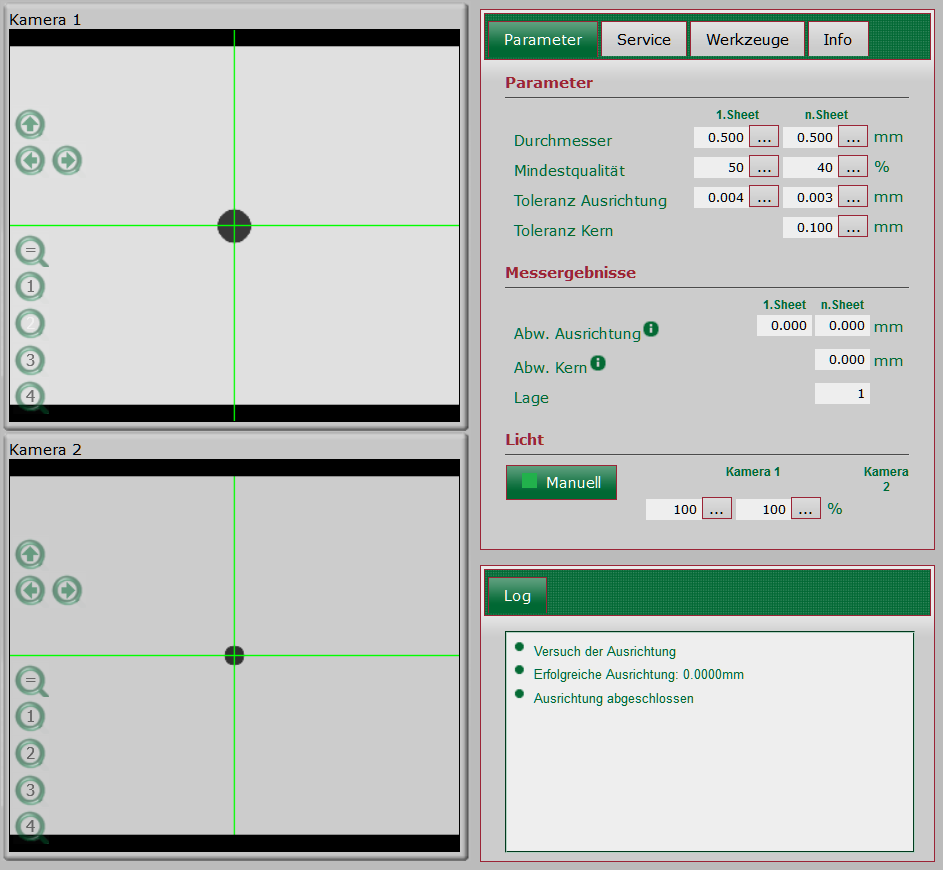
\includegraphics[width=\textwidth, height=\textwidth]{media/webinterface-alt.png}
		\caption{Interface vor dem Redesign}
		\label{fig:ivs-webinterface-alt}
	\end{minipage}
	\begin{minipage}{0.5\textwidth}
		\centering
		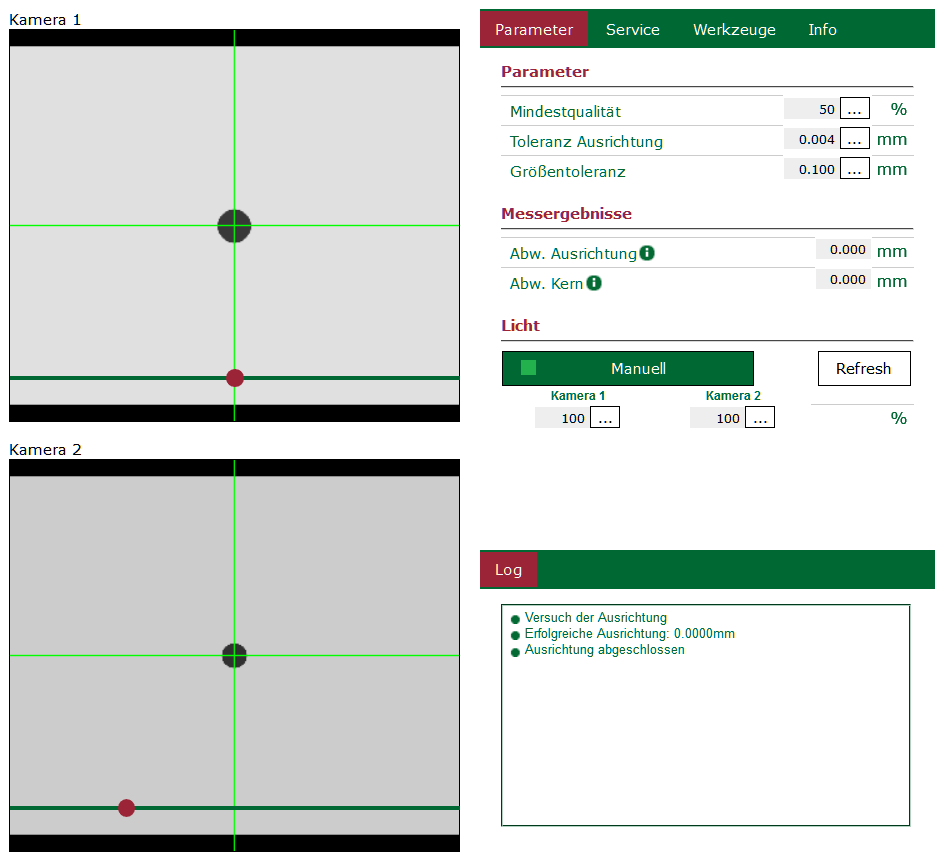
\includegraphics[width=\textwidth, height=\textwidth]{media/webinterface.png}
		\caption{Interface nach dem Redesign}
		\label{fig:ivs-webinterface}
	\end{minipage}
\end{figure}

\subsection{Javascript-Framework}
\label{subsec:ivs-einlesen-javascript}

In der bereits vorhandenen Version der Webseite wurde sämtliche Funktionalität durch
ein Javascript-Framework geregelt, welches unabhängig von Inhalt und Design steht.
Im Folgenden ging es nun darum, den hier geschriebenen Code durchzugehen, zu verinnerlichen
und zu verstehen.

Aufgrund der trotz weniger Codezeilen doch sehr hohen Komplexität und vor allem
den fehlenden Kommentaren gestaltete es sich als sehr schwierig, sich einzuarbeiten.
Ein weiterer Nachteil war meine mangelnde Erfahrung mit Javascript; durch viel Recherche
und weiterführende Beispiele konnte ich mir jedoch einiges herleiten und somit verstehen.

Weitere Modifikationen am Framework umfassten vor allem die Vereinfachung und Lesbarkeit
des Codes. Die Hauptaufgabe in dieser Phase war das Verständnis, da dies die Grundlage
für weitere Arbeit am Javascript war.



\section{Dokumentation des Frameworks}
\label{sec:ivs-dokumentation}

Eine weitere wichtige Aufgabe war das Dokumentieren des bereits vorhandenen Codes.
Da der ursprüngliche Autor leider nicht mehr bei isys vision angestellt war und
ich mich nun schon länger damit auseinander gesetzt hatte, sollte nun eine umfassende
Dokumentation des Aufbaus erstellt werden.

Dies erleichtert einerseits die Arbeit am Framework selbst (Änderungen und Updates
beispielsweise) und bietet denjenigen, die es nur verwenden (z.B. für eine neue
Webseite mit demselben Framework) ein einfaches, gut verständliches Interface. Weiterhin
können komplexere Vorgänge wie die Datenübertragung anschaulich erklärt und mithilfe
von Diagrammen verdeutlicht werden.


\subsection{Codekommentierung mit JSDoc}
\label{subsec:ivs-dokumentation-jsdoc}

Im ersten Schritt arbeitete ich dabei nur am Quelltext selbst, den ich zuvor schon
in lesbare Form gebracht hatte. Durch zusätzliche Kommentare an wichtigen und irreführenden
Stellen konnte ich dabei eine erste Grundlage schaffen. Die größte Änderung war
die Einführung einer Codedokumentation im \texttt{JSDoc}-Format\footnote{\url{https://en.wikipedia.org/wiki/JSDoc}},
ähnlich zu den bei Java eingesetzten JavaDoc-Kommentaren. Die Vorteile davon liegen
auf der Hand: Jede Methode bzw. Funktion hat somit eine eigene Beschreibung, in
der Funktionsweise, Parameter, Rückgabewert usw. beschrieben werden.

Ein weiterer Vorteil von JSDoc ist die Möglichkeit, die Dokumentation automatisch
zu generieren. Dies ist mit dem JSDoc-Tool von \texttt{Node.js} möglich, was nach
der Installation einfach über den Befehl \texttt{jsdoc file.js} aufgerufen kann.
Somit wird ein gut strukturiertes Dokument (inklusive Referenzen) automatisch erstellt.


\subsection{Beschreibung der API}
\label{subsec:ivs-dokumentation-beschreibung}

Nachdem der Quellcode selbst dokumentiert war, konnte ich mich nun mit den internen
Abläufen des Frameworks beschäftigen und diese anhand von Grafiken anschaulich machen.
In diesem Fall ging es vor allem um die Daten- und Befehlsübertragung vom IVS zum
Webinterface und umgekehrt.

Die Übertragung der Daten erfolgt hierbei über eine \texttt{XMLHttpRequest}, bzw.
(bei älteren Browsern) über ein \texttt{ActiveXObject}. Die Befehlscodes sind dabei
im HTML-Code der betreffenden Buttons gespeichert:

\begin{code}[language=html, caption={Ins HTML eingebettete Befehle für das IVS}, label={lst:ivs-html-befehle}]
<input type="text" size="6" maxlength="6" name="lms/SheetF.MinQuality">
<button name="lms/Cmd" value="10">Ausrichtung</button>
<button name="lms/Cmd" value="20">
	<ul>
		<li>LmsScb/Mot.RefOk</li>
		<li>Referenzfahrt</li>
	</ul>
</button>
\end{code}

In Zeile 1 wird beispielsweise das Register \texttt{lms/SheetF.MinQuality} geschrieben
und auf einen sechsstelligen Wert gesetzt, der vom Nutzer eingegeben wird.\\
In Zeile 2 befindet sich ein einfacher Befehlsbutton, der den Wert \texttt{10} ins
Register \texttt{lms/Cmd} schreibt (beim IVS ist dies der Code für eine Ausrichtung).\\
In den Zeilen 3 - 8 findet sich nun ein Knopf mit Status, der
\begin{itemize}
	\item den Wert \texttt{20} ins Register \texttt{lms/Cmd} schreibt und somit eine
	Referenzfahrt auslöst
	\item innerhalb der unsortierten Liste (Zeile 5) den Wert \texttt{LmsScb/Mot.RefOk}
	liest (Status der Referenzfahrt).
\end{itemize}
Die Liste (\texttt{<ul>}) dient dabei ausschließlich der Darstellung und hat keine
Auswirkung auf die Funktion; die Listenelemente werden innerhalb des Buttons entsprechend
formatiert. Weiterhin wird je nachdem, was im gelesenen Register \texttt{LmsScb/Mot.RefOk}
steht, ein entsprechendes Label gesetzt (grün falls Referenzfahrt OK, rot falls
nicht).

Im Javascript-Framework wird nun ein Event-Listener für alle Buttons und Eingabefelder
erstellt, der dann die entsprechenden Befehle erkennt. Diese werden in Form einer
URL in einer Liste gespeichert, welche dann mithilfe der bereits genannten \texttt{XMLHttpRequest}
bzw. des \texttt{ActiveXObject}s ans IVS gesendet werden. Die Antwort des IVS wird
dann entsprechend weiterverarbeitet und beispielsweise in Form eines Kamerabildes
direkt ausgegeben.





%+-----------+
%| Kapitel 2 |
%+-----------+
\chapter{Integration von Jira und Confluence}
\label{ch:jira}

Das nächste größere Projekt war die Integration der Atlassian-Produkte \textit{Jira}\footnote{\url{https://de.wikipedia.org/wiki/Jira_(Software)}}
und \textit{Confluence}\footnote{\url{https://de.wikipedia.org/wiki/Confluence_(Atlassian)}} in den Firmenalltag. Diese beiden Programme sind für das
Production Management gedacht und haben das Ziel, einen durchgängigen, geplanten
und leicht nachvollziehbaren Arbeitsfluss zu erreichen.

Confluence ist dabei ein einfaches System, dessen Ziel die einfache Weitergabe von
Informationen ist. Es dient der Erstellung von Dokumenten, welche externe Daten
wie beispielsweise Microsoft-Office-Dokumente oder YouTube-Videos sowie Bilder usw.
enthalten können und vereinfacht die Zusammenarbeit mehrerer Personen an einem Dokument.

Jira arbeitet im Zusammenspiel mit Confluence und ist ursprünglich für die Softwareentwicklung
gedacht. Entwicklungsvorgehensweisen wie \textit{Scrum} o.Ä. können hier ohne Umwege
umgesetzt werden und Jira bietet Funktionalitäten wie Sprints oder Burndown-Charts
an, um den Arbeitsfluss zu sichern.

Die Verwendung von Jira und Confluence sollte das davor eingesetzte (und veraltete)
Tool \textit{easyPM} ersetzen, welches für die Planung von Aufgaben, Abläufen und
Verwaltung von Zeitspalten eingesetzt wurde. Informationen wie E-Mails, Anrufprotokolle
oder sonstige Daten waren hier jedoch dezentral, bzw. konnten nicht direkt in easyPM
gespeichert werden. Durch das Zusammenspiel der beiden neuen Systeme sollte dieses
Problem behoben und die Speicherung der Daten konsistent werden.



\section{Einrichtung der Datenbank}
\label{sec:jira-einrichtung-datenbank}

Jira und Confluence sind beides Tools, die über einen Server laufen und dann über
den Webbrowser der Endgeräte aufgerufen werden können. Dies sichert zum einen die
Zentralität der Datenspeicherung und -verarbeitung und entlastet andererseits die
Nutzergeräte stark. Weiterhin ist die Nutzung eines firmeninternen Servers (welcher
außerdem für andere Zwecke wie das Intranet schon vorhanden war) sinnvoll, da somit
die Sicherheit der gespeicherten Daten gewährleistet wird.

Für den Aufbau des Webservers wird dabei sowohl von Jira als auch von Confluence
eine Datenbank verwendet. Das kann sowohl eine \textit{MySQL}-, \textit{Oracle}-
oder \textit{Microsoft-SQL}-Datenbank sein, oder aber auch die Open-Source-Alternative
\textit{PostgreSQL}. Wegen der eher schlechten Unterstützung von MySQL habe ich
schlussendlich eine PostgreSQL-Datenbank eingesetzt.

PostgreSQL ist ein freies und quelloffenes Datenbankmanagementsystem. Es wird von
Betriebssystemen wie Windows, Linux und anderen UNIX-ähnlichen Systemen unterstützt
und wird bei den meisten Linux-Distributionen bereits mitgeliefert.

Um den Linux-Server von isys zu simulieren und die Datenbank entsprechend einzurichten,
habe ich eine virtuelle Maschine mit einer Ubuntu-Installation verwendet. Nach der
Einrichtung des Systems konnte ich mit der Konfiguration des Datenbankservers beginnen.
Nach einiger Verwirrung und etwas Recherche stellte sich heraus, dass für das Erstellen
einer Tabelle in PostgreSQL\footnote{\url{https://de.wikipedia.org/wiki/PostgreSQL}} ein Linux-Nutzername angegeben werden muss. Dies war
praktisch, da die Jira- und Confluence-Systemdienste sowieso einen eigenen Account
erstellten, den ich somit direkt mitverwenden konnte. Ich hatte nun also drei Zugänge:

\begin{itemize}
	\item \texttt{ubuntu}, Super-User-Account und Hauptaccount des Rechners,
	\item \texttt{confluence}, für die Datenbank und den Systemdienst des Confluence-Servers,
	\item \texttt{jira}, für die Datenbank und den Systemdienst des Jira-Servers.
\end{itemize}

Mit einigen einfachen SQL-Befehlen waren die notwendigen Datenbanken dann auch schnell
erstellt:

\begin{code}[language=SQL, caption={SQL-Befehle zur Erstellung der Datenbanken}, label={lst:jira-database}]
CREATE DATABASE confluencedb WITH ENCODING 'UNICODE';
GRANT ALL PRIVILEGES ON DATABASE confluencedb TO confluence;

CREATE DATABASE jiradb WITH ENCODING 'UNICODE';
GRANT ALL PRIVILEGES ON DATABASE jiradb TO jira;
\end{code}

Zur Anbindung an Jira bzw. Confluence musste nun nur noch bei der Einrichtung jeweils
die entsprechenden Datenbankdaten angegeben werden. Da hier der Jira- bzw. Confluence-Server
und die Datenbank auf dem selben Rechner laufen, ist der Host beispielsweise \texttt{127.0.0.1}
bzw. \texttt{localhost}.

Die Installation von Jira und Confluence erfolgte dann einfach über die Ausführung
eines Shell-Skriptes und die Eingabe einer Lizenz. Somit war die Einrichtung der
Systeme vollständig und ich konnte einige Einstellungen vornehmen, z.B. Anpassungen
im Design der Seiten, sodass die Oberfläche den Farben der Firma entsprach
(\textcolor[HTML]{006833}{Grün [\texttt{\#006833}]} und \textcolor[HTML]{9B2536}{Rot [\texttt{\#9B2536}]}).



\section{Einrichtung des Intranetservers}
\label{sec:jira-server}

Nun, da Jira und Confluence online und konfiguriert waren, setzte ich mich mit der
Einrichtung eines Servers auseinander, welcher im Intranet betrieben werden und
die beiden Webtools hosten sollte.

Im ersten Schritt machte ich den dafür zur Verfügung gestellten Rechner nutzbar,
indem ich eine frische Linux-Installation vornahm. Auf dieser Basis konnte ich nun
mit \texttt{VirtualBox}\footnote{\url{https://wiki.ubuntuusers.de/VirtualBox/Installation/\#VirtualBox-OSE-Open-Source-Edition}}
eine virtuelle Maschine einrichten; auch darauf lief ein Linux-Betriebssystem. Die
Nutzung einer virtuellen Maschine hatte hierbei mehrere Vorteile:

\begin{enumerate}
	\item \textbf{Flexibilität}:
	Durch das Speichern in einem \textbf{Disk Image}\footnote{\url{https://de.wikipedia.org/wiki/Speicherabbild}} ist der Ort des Servers
	sehr leicht austauschbar. Durch Verschieben des Images sind sämtliche Daten des
	Servers übernommen, was die Wartung stark vereinfacht.
	\item \textbf{Sicherheit}:
	Da die Daten in einem einzigen Image liegen, welches auf der Festplatte des
	Wirtrechners gespeichert wird, ist die Datensicherung bzw. Erstellung von Backups
	besonders komfortabel. Mithilfe eines RAID-Systems wird in diesem Fall die Datensicherheit
	gewährleistet und Backups erstellt.
	\item \textbf{Vielseitigkeit}:
	Der Server läuft in einer virtuellen Maschine, welche auf die Ressourcen
	des Wirtrechners zugreift. Durch das Einrichten einer weiteren virtuellen Maschine
	kann dessen Rechenleistung und Speicherkapazität optimal ausgenutzt werden und
	die Maschine somit auch für andere Zwecke verwendet werden.
\end{enumerate}

Nach erneuter Einrichtung der in Kapitel \ref{sec:jira-einrichtung-datenbank} beschriebenen
Datenbank und der Anbindung an Jira/Confluence musste ich mich nun noch mit der
Netzwerkverbindung auseinandersetzen. Die zugeordnete IP-Adresse sollte dabei
\texttt{10.0.0.14} sein; Jira und Confluence jeweils unter den Standardports
\texttt{8080} bzw. \texttt{8090} erreichbar sein.

Als Erstes musste die virtuelle Maschine über eine Netzwerkbrücke auf das lokale
Netzwerk zugreifen können. Dies war schnell eingestellt; eine einfache Änderung
im VirtualBox-Interface genügte dafür. Mithilfe der Netzwerkbrücke wird hier das
lokale Netzwerk (isys vision Intranet) mit dem von der virtuellen Maschine erstellten
Netzwerk verbunden, sodass diese die gehosteten Services auf die Webports anlegen
kann.

Im nächsten Schritt braucht die virtuelle Maschine eine feste (statische) IP-Adresse.
In diesem Fall sollte dies die \texttt{10.0.0.14} sein. Um diese zuzuweisen, kann
unter Linux die Datei \texttt{/etc/network/interfaces} bearbeitet werden:

\begin{code}[language=bash, caption={Änderungen in \texttt{/etc/network/interfaces}}]
auto enp0s3 #Name der Netzwerkbrücke
iface enp0s3 inet static #IP auf Statisch ändern
#Setzen von Verbindungsinformationen
netmask 255.255.0.0
gateway 10.0.0.10
network 10.0.0.0
broadcast 10.0.0.255
dns-nameservers 10.0.0.10
\end{code}

Mithilfe dieser Änderungen wird dem Rechner eine statische Adresse zugewiesen. Dies
ist hier notwendig, da der Rechner sonst bei jedem Start vom Router eine neue, variable
Adresse zugewiesen bekommt. Damit der Server also immer mit der selben Adresse erreichbar
ist, muss die IP fest sein. Später lässt sich auch eine DNS zuweisen, beispielsweise
\texttt{intranet.isys-vision.de/jira}.



\section{Ausfallsicherheit über ein RAID-System}
\label{sec:jira-raid}

Um die Stabilität des Servers im Intranets zu gewährleisten, sollte das System durch
ein RAID-5\footnote{\url{https://de.wikipedia.org/wiki/RAID\#RAID\_5}} abgesichert
werden. Ein RAID-5 besteht aus mindestens 3 unabhängigen Festplatten, welche dieselben
Daten redundant abspeichern. Beim Ausfall einer der Platten wird somit sichergestellt,
dass die Daten weiterhin verfügbar (und auch nutzbar) bleiben.

Da Hardware-RAIDs oft sehr teuer sind, habe ich auf ein Software-RAID zurückgegriffen.
Hierbei wird die Redundanz der Daten durch Software erreicht, welche das Plattenmanagement
übernimmt. Das Betriebssystem verblieb dabei auf der vorherigen Platte, sodass nur
die virtuelle Maschine auf dem RAID gespeichert wird.

Unter Linux lässt sich ein RAID mit dem Tool \texttt{mdadm} sehr gut realisieren.
Man kann dabei auswählen, welches RAID-Level gewählt (in diesem Fall ein RAID-5-System)
und welche und wie viele Festplatten genutzt und werden sollen. Dazu reicht ein
einziger Befehl aus:
\begin{code}
sudo mdadm --create --verbose /dev/md0 --level=5 --raid-devices=3 /dev/sdb /dev/sdc /dev/sdd
\end{code}
\texttt{/dev/sdb}, \texttt{/dev/sdc} und \texttt{/dev/sdd} sind die Festplatten,
die genutzt werden sollen. Unter \texttt{/dev/md0} wird nach Abschluss des Vorgangs
das neue ``Gerät'' liegen, es lässt sich wie eine einzelne Festplatte behandeln.
Das System wird nun eingerichtet, und mithilfe von
\begin{code}
cat /proc/mdstat
\end{code}
kann man den aktuellen Status ansehen. Das Einrichten dauert je nach Festplattengeschwindigkeit
und -größe sehr lange.

Nach Abschluss dieser Einrichtung muss ein Dateisystem für die Festplatten festgelegt
werden. Unter Linux wird standardmäßig das Ext4-System verwendet. Es lässt sich mit
\begin{code}
sudo mkfs.ext4 -F /dev/md0
\end{code}
installieren. Weiterhin muss ein Einhängepunkt für die Festplatte erstellt werden
(also ein Verzeichnis im Dateisystem, von dem aus darauf zugegriffen werden kann).
Dies geschieht mit
\begin{code}
sudo mkdir /media/md0
\end{code}
Durch einen entsprechenden Eintrag in der Datei \texttt{/etc/fstab} kann die Festplatte
nun beim Systemstart automatisch eingehängt werden. Die neue Zeile lautet
\begin{code}
/dev/md0 /media/md0 ext4 defaults 0 2
\end{code}
In der ersten Spalte wird der Ort der Festplatte angegeben, danach der Einhängepunkt.
Es folgen das Dateisystem und weitere Optionen (defaults reicht hier aus).

Das RAID-System ist nun vollständig konfiguriert. Nach einem Neustart des Computers
kann das Speicherabbild der virtuellen Maschine nun darauf gespeichert und die Daten
somit ausfallsicher gemacht werden.


%+-----------+
%| Kapitel 3 |
%+-----------+
\chapter{Web-Tools für das Mikado-Projekt}
\label{ch:webtools}

Nach meiner Arbeit am IVS, Jira und Confluence wurde ich nun Teil eines anderen
Projekts namens Mikado\footnote{\url{http://www.mikado-robotics.de}}. Mikado ist ein Robotikprojekt,
bei dem es hauptsächlich um das sogenannte ``Bin Picking'' geht. Dabei wird ein
Roboter dazu eingesetzt, zufällig in einer Kiste liegende Teile mithilfe einer 3D-Kamera
zu erkennen, zu greifen und in eine andere Position zu bringen. Die Herausforderung
liegt hierbei beim Leeren der Kiste, d.h. alle sich darin befindlichen Teile gleichgültig
ihrer Position greifen zu können.

\begin{figure}[H]
	\begin{center}
		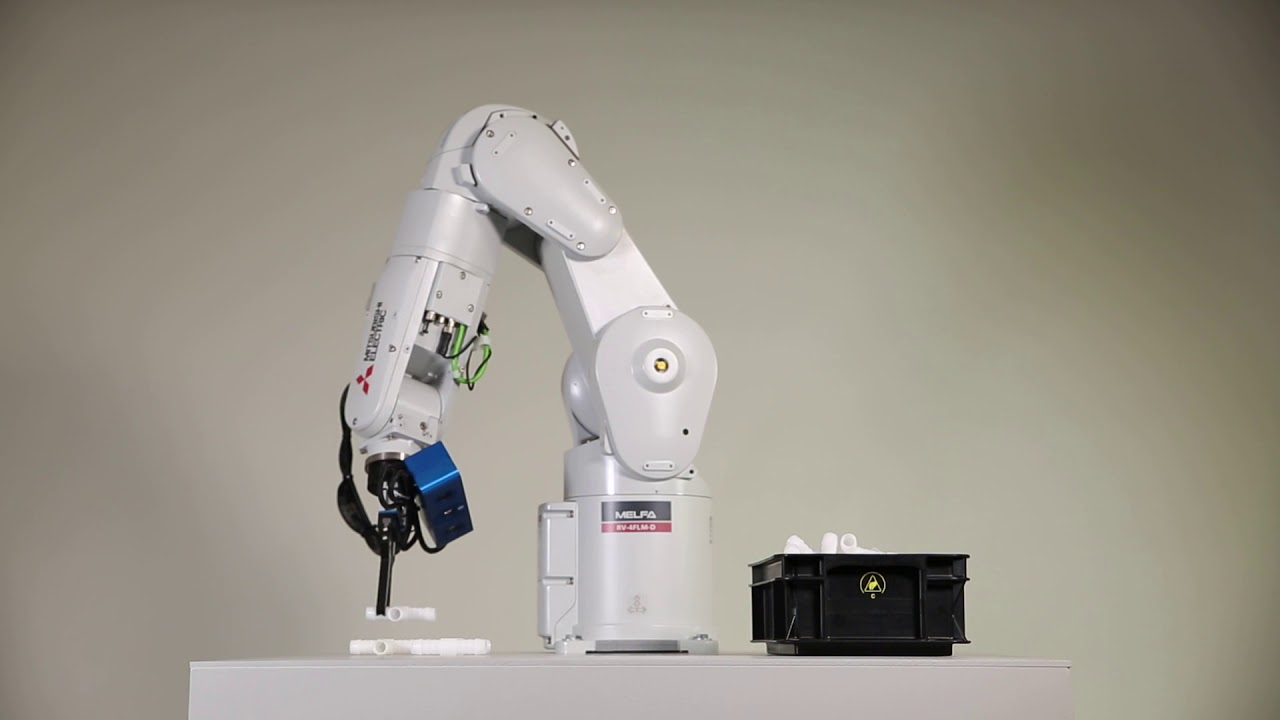
\includegraphics[width=0.75\textwidth]{media/mikado-roboter.jpg}
		\caption[Mikado-Roboter von Misubishi]{Mikado-Roboter von Mitsubishi\footnotemark}
		\label{fig:mikado-roboter}
	\end{center}
\end{figure}
\footnotetext{Quelle: \url{https://img.youtube.com/vi/L7nppfZ6pKg/maxresdefault.jpg}}



\section{Demoablauf für Messen}
\label{sec:webtools-demo}

Zum Kennenlernen der Programmschnittstelle und des Roboters sollte ich zunächst
mit dem von isys geschriebenen Programm einen Demoablauf aufbauen, welcher für
Messen oder ähnliche Anwendungsfälle verwendet werden sollte. Im Programm lassen
sich dafür Abläufe graphisch regeln, beispielsweise eine Bewegung, das Greifen
eines Teils oder die Bildaufnahme mit der 3D-Kamera. Diese noch nicht veröffentlichte
Software konnte somit außerdem von mir getestet und Verbesserungsvorschläge geäußert
werden.

Zur Erkennung der Teile wird mithilfe der Kameras ein 3D-Bild aufgenommen, welches
anschließend von der Recheneinheit analysiert und zu einer Punktwolke transformiert
wird. Diese Punktwolke wird nun mit dem eintrainierten CAD-Modell abgeglichen und
somit mögliche Kandidaten anhand ihrer Übereinstimmung identifiziert. Die dabei
gewählte Mindestübereinstimmung lässt sich dabei einstellen, was je nach Wert
Vor- bzw. Nachteile mit sich bringt:

\begin{table}[H]
	\begin{tabular}{| l || l |}
	\hline
	\textbf{Höhere Mindestqualität} & \textbf{ Niedrigere Mindestqualität}\\
	\hline\hline
	Erkannte Teile können mit höherer Sicherheit & Erkannte Teile können sich in nahezu un-\\
	richtig und sicher gegriffen werden & greifbarem Winkel befinden und daher nicht\\
	& sicher gegriffen werden\\
	\hline
	Weniger Teile werden erkannt, daher höhere & Viele Teile werden erkannt, die Wahrschein-\\
	Chance, die Kiste nicht leer zu bekommen & lichkeit ist daher größer, alle verbleibenden\\
	& Teile zu identifizieren\\
	\hline
	\end{tabular}
	\caption{Vor- bzw. Nachteile einer höheren vs. niedrigeren Mindestqualität}
	\label{tab:webtools-demo-mindestqualität}
\end{table}

Die Bewegungen des Robotors lassen sich entweder über die Winkel der einzelnen Gelenke
(beim von isys verwendeten Roboter von Mitsubishi Electrics sind es 6 Gelenke) oder
das Format \texttt{xyz rpy} (\texttt{xyz} ist hierbei die Position im Raum (3 Koordinaten),
\texttt{rpy} (roll, pitch, yaw) die Drehung des Greifers) angeben. Sämtliche Bewegungen
und Rotationen sind dabei kollisionsgeprüft, d.h. sobald das System eine mögliche
Kollision erkennt, wird die Bewegung nicht ausgeführt. In diesem Fall kann eine
alternative Aktion durch einen Sprung im Programmablauf durchgeführt werden.

Über einzelne Sektionen und Sprünge lässt sich nun ein strukturiertes Programm erstellen,
was sowohl einfache Funktionen (wie in diesem Fall eine Demonstration der Funktionalität)
oder auch komplexe Abläufe wie den Zusammenbau eines Schneckengewindes übernehmen
kann. Der Programmablauf kann dabei mit den Funktionen \texttt{start}, \texttt{pause},
\texttt{step} und \texttt{reset} gesteuert werden, was in folgenden Aufgaben noch
wichtig wird.

Mein Demonstrationsprogramm war hierbei die Abwandlung einer älteren Demo. Der Roboter
nimmt dabei Zahnräder aus einer Kiste, testet mithilfe einer Lichtschranke, ob er
das Teil tatsächlich gegriffen hat, und legt dieses schlussendlich so ab, dass der
Schriftzug ``isys'' entsteht. Ist dies geschehen, nimmt er nacheinander die abgelegten
Teile wieder auf und legt sie zurück in die Kiste.

Der Zweck der Demonstration ist einerseits das Heranführen an den Roboter an sich
(z.B. die Arbeitsweise der Maschine oder die graphische Programmierung) sowie die
Fähigkeit, wirklich sämtliche Teile aus der Kiste nehmen zu können, zu demonstrieren.
Erreichen lässt sich dies einfach dadurch, dass zu Beginn nur so viele Zahnräder
in die Kiste gelegt werden, wie am Ende auch für den Schriftzug benötigt werden.



\section{Web-Remote für die Mikado-Software}
\label{sec:webtools-remote}

Für die Demonstration bei Messen oder bei ähnlichen Veranstaltungen sollte nun von
mir ein Webinterface erstellt werden, was als Fernzugriff für die Mikadosoftware
verwendet werden kann. Der Sinn dahinter ist, dass der Programmablauf nicht mehr
ausschließlich mithilfe von Bildschirm und Tastatur gesteuert, sondern beispielsweise
über ein Smartphone modern und komfortabel bedient werden soll. Dies ist insbesondere
nützlich, da aus Sicherheitsgründen bei Vorführungen eine Glaswand vor dem Roboteraufbau
ist, was Eingriffe in den Ablauf stark erschwert.


\subsection{Design der neuen Webseite}
\label{subsec:webtools-remote-design}

Nachdem ich im \ref{ch:ivs}. Projekt bereits mit Javascript, CSS und HTML in Berührung
gekommen war, konnte ich nun eine völlig neue Webseite basierend auf meinen erlangten
Kenntnissen selbstständig und von Grund auf aufbauen. Dazu kümmerte ich mich zuerst
um Inhalt und Design der neuen Seite und fügte anschließend die Funktionalität durch
Javascript und jQuery hinzu.

\subsubsection{Struktur mit HTML}
\label{subsubsec:webtools-remote-design-html}

Zunächst gliederte ich die neue Webseite mithilfe der zugehörigen HTML-Tags in sinnvolle
Abschnitte. Mit \texttt{<nav>}, \texttt{<main>} und \texttt{<footer>} sowie geschachtelten
\texttt{<div>}-Tags konnte ich eine sinnvolle Struktur in den Inhalt der Seite bringen.

Im \texttt{<nav>}-Teil der Seite wird die Navigationsleiste definiert; in meinem
Fall umfasste sie die Listenpunkte \textbf{Logs}, \textbf{Kontrolle} und \textbf{Über}
sowie ein \textbf{Hamburger-Menü-Icon}\footnote{\url{https://de.wikipedia.org/wiki/Hamburger-Men\%C3\%BC-Icon}},
welches zum Ein- und Ausklappen des Menüs notwendig war. Im \texttt{<main>}-Teil
des HTML-Dokuments wird sämtlicher Inhalt der Seite definiert, also in meinem Fall
das Logfenster, die Kontroll- und die Informationsseite. Diese einzelnen Abschnitte
sind jeweils wieder in einzelne \texttt{<div>}s geteilt, sodass Struktur und Design
gewährleistet werden können. Schlussendlich befinden sich im \texttt{<footer>}-Element
einige Informationen über das Produkt, wie z.B. Copyright, Webseite oder Kontakt.

\begin{code}[language=html, caption={Struktur der Kontrollseite}]
<div id="control" class="content">
	<div class="control-window">
		<div class="control-element">
			<button onclick="start()">
				<img src="media/start.svg" alt="Start">
			</button>
		</div>
		<div class="control-element">
			<button onclick="step()">
				<img src="media/step.svg" alt="Step">
			</button>
		</div>
		<div class="control-element">
			<button onclick="pause()">
				<img src="media/pause.svg" alt="Pause">
			</button>
		</div>
		<div class="control-element">
			<button onclick="reset()">
				<img src="media/reset.svg" alt="Reset">
			</button>
		</div>
	</div>
</div>
\end{code}

Wie man sieht, bestehen die Kontrollbuttons aus einem Funktionsaufruf (den ich erst
später implementiert habe) und einer SVG-Grafik\footnote{\url{https://de.wikipedia.org/wiki/Scalable\_Vector\_Graphics}}.

\subsubsection{Erstellen von SVG-Grafiken}
\label{subsubsec:webtools-remote-design-svg}

SVG-Grafiken haben den großen Vorteil, dass sie vom Browser gerendert werden. Dadurch
ist einerseits keine große Bilddatei notwendig, was (insbesondere auf mobilen Endgeräten)
zu sehr schnellen Ladezeiten führt, und andererseits auch nicht das Problem zu geringer
Auflösungen mit sich bringt, wodurch die Grafik immer gestochen scharf ist. Da jedoch
keine entsprechenden Grafiken vorhanden waren, musste ich diese selbst erstellen.
Auch für das Navigationsmenü habe ich SVG-Dateien entworfen.

Der Inhalt einer SVG-Grafik ist der Syntax von HTML bzw. XML sehr ähnlich. Zunächst
wird mit dem Tag \texttt{<svg>} gekennzeichnet, dass es sich um eine SVG-Grafik
handelt. Innerhalb dieses Tags können nun Bildelemente hinzugefügt werden:

\begin{code}[language=svg, caption={Bildelemente in einer SVG-Grafik}]
<svg width="54" height="54" viewBox="0 0 54 54" xmlns="http://www.w3.org/2000/svg" xmlns:xlink= "http://www.w3.org/1999/xlink">
	<circle
		cx="27" cy="27" r="25"
		stroke="black" stroke-width="4" fill="none"
	/>
	<line
		x1="18" y1="13"
		x2="18" y2="41"
		stroke="black" stroke-width="8" stroke-linecap="butt"
	/>
	<line
		x1="36" y1="13"
		x2="36" y2="41"
		stroke="black" stroke-width="8" stroke-linecap="butt"
	/>
</svg>
\end{code}

Hier wird beispielsweise zunächst ein umschließender Kreis definiert (ll. 2 - 5),
welcher den Mittelpunkt $P(27|27)$ und den Radius $r = 25$ hat. Die Linienfarbe
soll Schwarz sein, die Linienbreite 4 Pixel und der Kreis soll nicht gefüllt sein.
Anschließend werden zwei Linien gezeichnet, jeweils mit der Farbe Schwarz, der Breite
8px und einem geraden Linienende. Linie 1 geht in diesem Fall von $P(18|13)$ nach
$Q(18|41)$.

\subsubsection{Stilregeln durch CSS}
\label{subsubsec:webtools-remote-design-css}

Im nächsten Schritt ging es um das Design mithilfe von CSS. Die vorhergehend definierten
Inhalte konnte ich nun schöner Darstellen, indem ich Stilregeln für bestimmte Elemente
und Klassen vornahm. Dazu gehörten unter Anderem die Schriftart, Farbschema für
Menüleiste und Links oder auch Positionierung von Abschnitten und Festlegen von
Abständen.

Sehr wichtig war hierbei die Orientierung an relativen Werten wie der Bildschirmweite
(\texttt{viewport width}). Da es sich hierbei um ein für Mobilgeräte optimiertes
Webinterface handelt, spielt Skalierbarkeit auf unterschiedliche Größen eine große
Rolle. Umsetzen lässt sich dies beispielsweise durch ein sogenanntes \textbf{Responsive
Design}\footnote{\url{https://de.wikipedia.org/wiki/Responsive_Webdesign}}, bei dem
die Webseite der Bildschirmgröße entsprechend reagiert. Dies sichert auch eine gute
und intuitive Darstellung beim Wechsel vom Portrait- in den Landschaftsmodus (z.B.
bei Tablet PCs).

In der Umsetzung erfolgt dies durch die Verwendung von relativen Werten (wie beispielsweise
\texttt{width: 1em;}) und \texttt{@media}-Tags, welche für die Skalierbarkeit der
Webseite und den enthaltenen Elementen verantwortlich sind.

\begin{figure}[H]
	\begin{center}
		\begin{minipage}{0.3\textwidth}
			\centering
			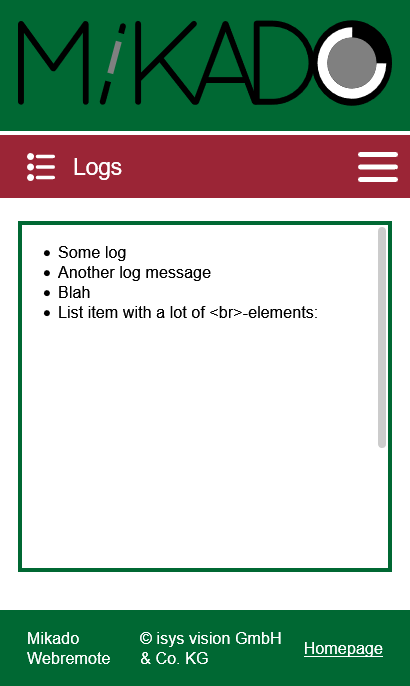
\includegraphics[width=\textwidth]{media/webremote-logs.png}
			\caption{Logfenster}
			\label{fig:webtools-remote-design-logfenster}
		\end{minipage}
		\begin{minipage}{0.3\textwidth}
			\centering
			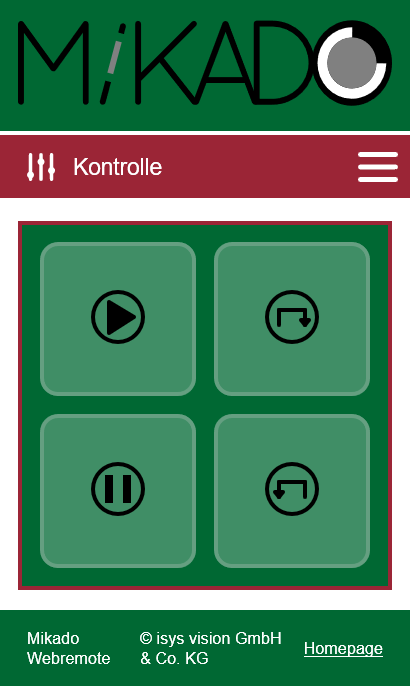
\includegraphics[width=\textwidth]{media/webremote-kontrolle.png}
			\caption{Kontrolle}
			\label{fig:webtools-remote-design-kontrolle}
		\end{minipage}
		\begin{minipage}{0.3\textwidth}
			\centering
			
\includegraphics[width=\textwidth]{media/webremote-info.png}
			\caption{Info / Menü}
			\label{fig:webtools-remote-design-info}
		\end{minipage}
	\end{center}
\end{figure}


\subsection{Befehls- und Logübertragung mithilfe von RoslibJS}
\label{subsec:webtools-remote-rosjs}

Auf dem Hostrechner des Roboters läuft zur Kontrolle von diesem eine Python-Bibliothek
namens ROS (Roboter Operating System). Sie bietet viele Funktionalitäten, beispielsweise
zum Steuern der einzelnen Gelenkwinkel durch Python.

Weiterhin werden Services zur Ausführung von einzelnen Aufgaben bereitgestellt.
Der Service \texttt{/reset} setzt beispielsweise den aktuellen Programmablauf
zurück und kann mit \texttt{rosservice call /reset} aufgerufen werden. Es sind
außerdem die Services \texttt{/run} und \texttt{/pause} vorhanden, welche die für
mich notwendige Funktionalität beinhalten. Die beiden letzteren werden mit Parametern
aufgerufen: \texttt{rosservice call /run ``step:false blocking:false''}, bzw.
\texttt{rosservice call /pause ``blocking:false''}.

Der Parameter \texttt{blocking} ist dabei in meinem Fall irrelevant; umso interessanter
ist jedoch das Argument \texttt{step}: Ist es auf \texttt{false} gesetzt, läuft
das Programm beim Aufruf normal durch. Sobald der Service jedoch mit \texttt{step:true}
aufgerufen wird, wird nur ein Schritt im Programmablauf durchgeführt.

Zur Anbindung an das von mir entwickelte Webinterface habe ich nun die Bibliothek
RoslibJS\footnote{\url{http://wiki.ros.org/roslibjs}} verwendet, welche als Kommunikationsmodul für ROS fungiert. Hiermit können
entsprechende Aufrufe im Javascript festgelegt werden, um diese anschließend an
den Hostrechner zu senden und somit den zugehörigen Service zu starten.

Meinen \texttt{<button>}-Elementen hatte ich jeweils die zugehörige Funktion im
Argument \texttt{onclick} zugeordnet (Beispiel: \texttt{<button onclick=''pause()''>Pause</button>}).
Im zugehörigen Javascript sind nun einmal die generelle Einrichtung von RoslibJS
(wie z.B. Verbindungsinformationen etc.) und für jeden Button die zugehörige Funktion
vorhanden.

\begin{code}[language=javascript, caption={Serviceaufruf durch RoslibJS}]
var ros = new ROSLIB.Ros();
ros.on('error', function(error) {/* Log weggelassen */});
ros.on('connection', function() {});
ros.on('close', function(){});
ros.connect('ws://10.0.4.136:8080');
/* Irrelevante Funktionen weggelassen */
function start() {
	var rosStart = new ROSLIB.Service({
		ros: ros, name: '/run', messageType: 'mikado_msgs/Run',
	});
	var rosStartRequest = new ROSLIB.ServiceRequest({
		step: false, blocking: false,
	});
	rosStart.callService(rosStartRequest);
}
/* Funktionsrumpf weggelassen */
function step() {};
function pause() {};
function reset() {};
/* Funktion zum Anhängen von Logs an das Logfenster. */
function initLog() {
	var rosLog = new ROSLIB.Topic({
		ros: ros, name: '/rosout', messageType: 'rosgraph_msgs/Log',
	});
	rosLog.subscribe(function(message) {
		var log = '<li class="';
		switch (message.level) {
			case 1:
				log += "debug";
				break;
		} //Other cases omitted
		log += '">' + message.msg + '</li>';
		addLog(log);
	});
}
\end{code}

Zunächst wird in den ersten 5 Zeilen die Verbindung zum ROS hergestellt. In den
anschließend folgenden Funktionen wird zunächst ein neuer Service für die aktuelle
Routine erstellt (Zeilen 8 - 12), welcher dann mit einer Anfrage (Zeilen 13 - 16)
gestartet wird (Zeile 17). Der Service selbst enthält hierbei Informationen über
den aufgerufenen Befehl (in diesem Fall \texttt{/run}), während die Anfrage Informationen
über die Parameter enthält (hier die Argumente \texttt{step} und \texttt{blocking}).

In der Funktion \texttt{initLog()} in Zeile 24 wird eine Verbindung zum ROS hergestellt,
um neue Lognachrichten ans Logfenster anzuhängen. Zunächst wird dafür ein sogenanntes
``Topic'' erstellt, welches dann mithilfe von \texttt{subscribe()} laufend aktualisiert
werden kann. Den hier ankommenden Nachrichten wird nun mithilfe des Wichtigkeitslevels
eine entsprechende CSS-Klasse zugewiesen (z.B. haben Meldungen vom Typ \textcolor[HTML]{006600}{\texttt{debug}}
die Farbe grün, \textcolor[HTML]{DD0000}{\texttt{error}} ist rot usw). Anschließend
werden die eigentlichen Logmeldungen an die bereits existierende Liste angehängt
und erscheinen somit im Logfenster.


\subsection{Webhosting und Netzwerk}
\label{subsec:webtools-remote-netzwerk}

Nachdem das Interface nun eigentlich die gewünschte Funktionalität besitzt, muss
es noch erreichbar gemacht werden. Dazu wird ein HTTP-Server verwendet, welcher
die Webseite hostet. Mit der Python-Bibliothek \texttt{flask} ist dies recht einfach
zu realisieren:

\begin{code}[language=python, caption={Python-Skript zum Hosten des Webservers}]
import rospy
from flask import Flask, render_template
app = Flask(__name__)
@app.route('/')
def render_static():
    return render_template('index.html')
if __name__ == '__main__':
    app.run()
\end{code}

Nun lässt sich unter der IP-Adresse des Rechners (lokal \texttt{127.0.0.1}) die
gehostete Webseite aufrufen. Über ein WLAN-Netzwerk lässt sich nun eine Verbindung
zu mobilen Endgeräten aufbauen, welche dann auf das Webinterface zugreifen und somit
den Roboter kontrollieren können.



\section{Web-Preview zur Darstellung von Punktwolken}
\label{sec:webtools-preview}

Zur Objekterkennung beim Mikado-Roboter wird von diesem mithilfe der 3D-Kamera eine
sogenannte Punktewolke aufgenommen - eine Ansammlung von Punkten, welche jeweils
mit ihren Koordinaten abgespeichert werden. Somit wird eine Art ``3D-Gitter'' erzeugt,
welches dann mit dem vogegebenen Modell verglichen werden kann.

Zur Veranschaulichung sollten diese Punktewolken nun mithilfe von Javascript in
einer einfachen Seite visualisiert werden. Zuvor wurde auf umständliche und veraltete Methoden zurückgegriffen, beispielsweise wurde ein Video aufgezeichnet und per Mail verschickt. Die Nutzung eines Javascript-Frameworks
ist hierbei sehr sinnvoll und komfortabel, da

\begin{enumerate}
	\item Daten sehr flexibel und schnell zur Nutzung im Webinterface exportiert werden können
	\item durch die Darstellung im Browser nahezu jedes Endgerät die Möglichkeit hat, die Webansicht zu nutzen
	\item das Framework auf einem Server von isys gehostet werden kann und dann für jeden Kunden eine unterschiedliche Simulation geladen werden kann
	\item keine Installation auf Seite der Kunden notwendig ist.
\end{enumerate}


\subsection{Rendering mit \texttt{THREE.js}}
\label{subsec:webtools-preview-rendering}

Zur Darstellung der Punktewolke habe ich \texttt{THREE.js}\footnote{\url{https://threejs.org/}}
verwendet. Dabei handelt es sich um ein Framework, welches auf OpenGL bzw. WebGL
basiert und Funktionalitäten zum Rendering von Objekten bereitstellt.

\begin{figure}[H]
	\centering
	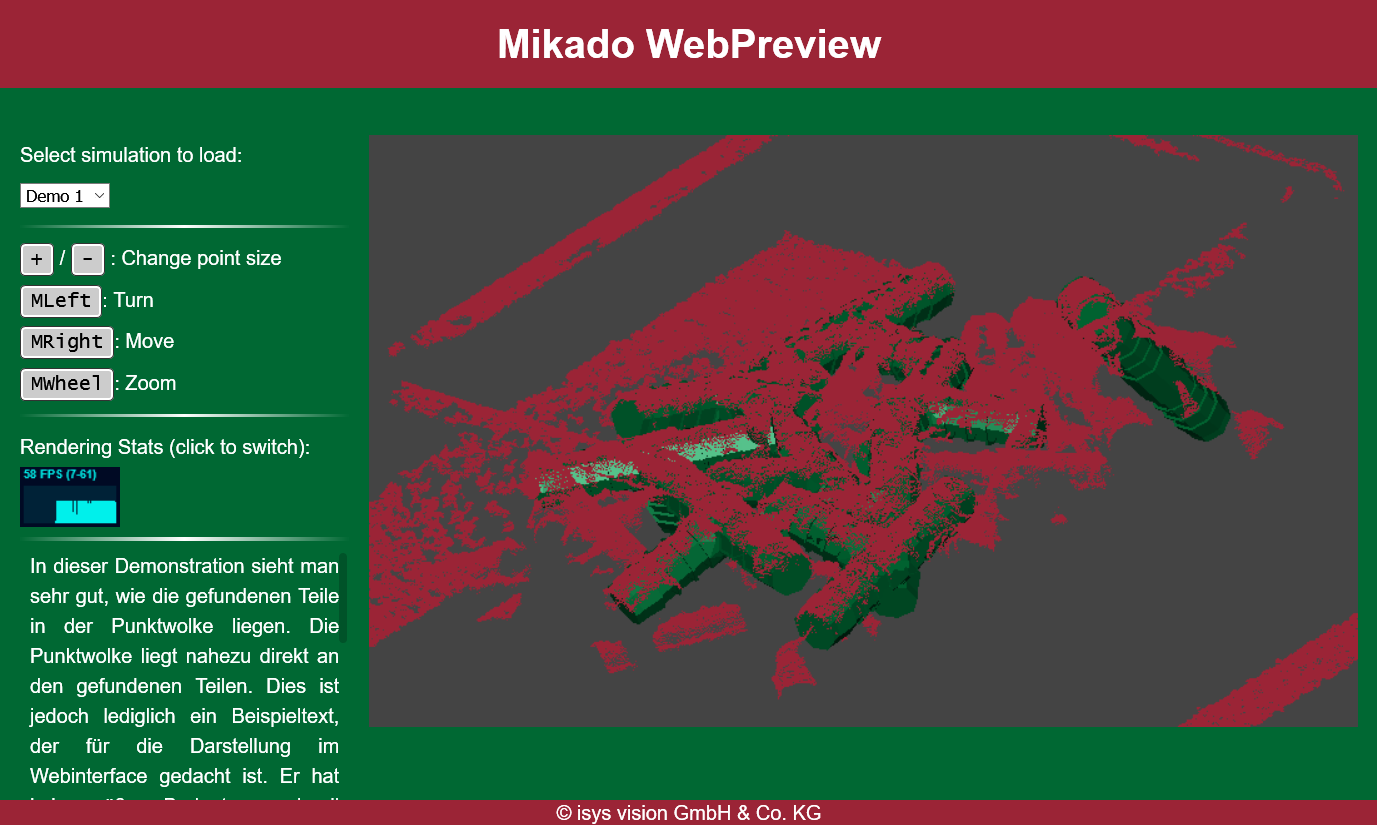
\includegraphics[width=0.75\textwidth]{media/webpreview.png}
	\caption{Punktwolke mit Beispielfunden in der Webvorschau}
	\label{fig:webtools-preview-rendering}
\end{figure}

Nachdem ein Grundgerüst aufgebaut wurde, welches THREE.js einbindet, kann der Renderer nun initialisiert werden. Das Framework
enthält dabei viele Methoden und Objekte, welche nun entsprechend deklariert und
genutzt werden können. Da es sich um viele kleine Konfigurationsschritte handelt,
ist folgendes Listing stark gekürzt.

\begin{code}[language=javascript, caption={Initialisierung von \texttt{THREE.js}}]
fetch('index.json');
function loadSTL(model, pose) { //Start loading found meshes
	fetch(pose); //Load position from .json file
	for (/*...*/) {
		scene.add(mesh); //Add meshes of found items
	}
}
function loadPCD(filename) {
	var pcdLoader = new THREE.PCDLoader(); //Load PCD file
	pcdLoader.load(filename /* material, position etc. omitted */);
}
function load() {
	/* create objects like renderer, scene, camera... */
}
function animate() {
	requestAnimationFrame(animate);
	renderer.render(scene, camera);
	controls.update();
}
function resizePoints(factor) {
	var pointCloud = scene.getObjectByName('pointcloud');
	pointCloud.material.size *= factor;
	pointCloud.material.needsUpdate = true;
}
\end{code}

Zunächst wird in Zeile 1 die Datei \texttt{index.json} geladen. Sie enthält wichtige Informationen wie eine Liste aus Punktwolken-Fundposition-Zusammenhängen sowie eine Beschreibung der Szene. Nachdem sie geladen wurde, werden Funktionen wie \texttt{load()} aufgerufen, die Simulation gestartet usw.

Die Funktionen \texttt{loadSTL} und \texttt{loadPCD} laden die \texttt{.stl}-Dateien der Funde bzw. die Punktwolke und setzen die in der JSON-Datei festgelegte Position der Teile. Sie werden bei Auswahl einer anderen Demo im Interface aufgerufen.

Die Funktion \texttt{load()} wird nun zur Initialisierung der Simulation aufgerufen und erstellt
einen Renderer, eine Szene (in der das Bild dargestellt wird) und die Kamera.

Die Funktion \texttt{animate()} ist eine einfache Update-Funktion, welche das
angezeigte Bild aktualisiert und mit jedem Frame aufgerufen wird. Hier wird
die Tastatureingabe gelesen bzw. auf einen relevanten Tastendruck gewartet.

In \texttt{resizePoints} wird die Größe der Punkte der Punktwolke geändert. Sie wird beim Tastendruck oder Klick auf einen Button im Interface aufgerufen.



\subsection{Konfiguration durch JSON-Dateien}

Das durch Bibliotheken und eigenes Javascript nun fertiggestellte Webtool sollte nun, je nach Kunde, mit unterschiedlichen Funddaten genutzt werden. In der Simulation sollte die Auswahl von festgelegten Demonstrationen durch ein Dropdown-Menü ermöglicht werden. Dafür wird in der Datei \texttt{index.json} eine Konfiguration erstellt, welche dann vom Javascript geladen, eingelesen und verwendet wird. Diese Datei enthält eine Liste von Demonstrationen. Sie besteht also aus mehreren Einträgen, welche dann als Optionen im Dropdown-Menü angezeigt werden.

\begin{code}[language=json,caption={Inhalt von \texttt{index.json}}]
[ {
	"pcd" : "pcdFile.pcd",
	"pcdColor" : "0x9b2436",
	"stl" : "stlFile.stl",
	"stlColor" : "0x006833",
	"pose" : "pose.json",
	"description" : ""
}, {} ]
\end{code}

Eine solche Option beinhaltet sechs Eigenschaften, deren Werte für die Darstellung verantwortlich sind:

\begin{itemize}
	\item pcd: Dateipfad zur Punktwolkendatei, die geladen wird.
	\item pcdColor: Die Farbe, in der die Punktwolke dargestellt wird.
	\item stl \& stlColor: analog zu den ersten beiden Eigenschaften.
	\item pose: Pfad zur JSON-Datei, welche Informationen über die Funde beinhaltet.
	\item description: Eine Beschreibung, die zusätzlich zur Animation angezeigt werden soll.
\end{itemize}

Die mit dem Namen ``pose'' gekennzeichnete Datei gibt dabei an, wie die STL-Modelle in der Punktwolke ausgerichtet werden. Sie beinhaltet sowohl Koordinaten der einzelnen Funde als auch die Rotation im Axis-Angle-Format\footnote{\url{https://en.wikipedia.org/wiki/Axis-angle_representation}}. Diese wird, wie auch die Punktwolke und Beschreibung, von isys-Mitarbeitern angelegt, und kontrolliert damit die Simulation. Die Informationen über das Fundstück, also die STL-Datei, stammen jedoch vom Kunden.


%+-----------+
%|   Fazit   |
%+-----------+
\chapter{Persönliche Bilanz und Ausblick}
\label{ch:fazit}

Während meiner Tätigkeit habe ich vielseitige Aufgaben und Probleme gelöst und konnte so in fast alle Unternehmensbereiche einen Einblick bekommen. Einerseits konnte ich mit den Entwicklern des IVS zusammenarbeiten und so einen Blick auf die teilweise noch sehr alte Technologie werfen. Im starken Gegensatz dazu war ich auch beim noch sehr jungen Mikado-Projekt aktiv und konnte damit die zukunftsorientierte Arbeitsweise des Unternehmens erfahren. Außerdem war ich bei der Einrichtung des Jira-Servers vollständig autonom, d.h. an keinem größeren Projekt direkt beteiligt. Hier habe ich die Technik im Production Management, Continuos Integration und der Versionsverwaltung kennengelernt.

Mit diesen Einblicken konnte ich mich sowohl fachspezifisch, fächerübergreifend als auch persönlich weiterbilden und viele wertvolle Erfahrungen sammeln. Besonders meine Fachkenntnisse zu Webentwicklung, insbesondere Javascript, konnte ich vertiefen. Außerdem wurde ich auch mit den Problemen der Entwicklung in Teams konfrontiert, beispielsweise der Wichtigkeit von korrekt dokumentiertem Code. Weiterhin erlangte ich einen Blick auf den Firmenalltag und Abläufe, was für mich neu war.

Die während meines Studiums erlangten Kenntnisse zu Datenbanken, Algorithmik und Programmiertechnik haben mir dabei stark weitergeholfen und mich gut auf die Arbeit im Unternehmen vorbereitet.

Besonders das weitreichende Aufgabenfeld und die freundschaftliche Beziehungen zu den Kollegen haben das Praktikum positiv geprägt. Mein einziger Kritikpunkt ist die lange Wartezeit, die ich zwischen verschiedenen Aufgaben hatte. Dies ist vermutlich jedoch auf die geringe Erfahrung der Firma mit studentischen Praktikanten zurückzuführen. Generell kann ich ein Praxissemester bei isys vision aber absolut empfehlen.


%+--------------------------+
%| Ehrenwörtliche Erklärung |
%+--------------------------+
\pagenumbering{gobble}
\chapter*{Ehrenwörtliche Erklärung}

Hiermit erkläre ich, dass ich den vorliegenden Bericht selbstständig angefertigt und alle von mir genutzten Quellen und Hilfsmittel angegeben habe. Dieser Bericht wurde bisher in keiner anderen Prüfungsbehörde oder Person im Rahmen einer Prüfung vorgelegt und auch nicht veröffentlicht.

\vspace{5cm}

\rule{3.5cm}{1pt} \hspace{1.5cm} \rule{10cm}{1pt}\\
Datum \hspace{4cm} Unterschrift\\



%+==============+
%| DOCUMENT END |
%+==============+
\end{document}
